\subsection{Konzept}
Aus Perspektive der Benutzer ist die Idee hinter StreamSwipe trivial. Dem User werden nacheinander Filme und Serien vorgeschlagen, die er bewerten kann. Auf Basis seiner Präferenzen erhält er Matches, mit denen er über eine Chatfunktionen kommunizieren kann. Jeder dieser Schritte muss möglichst schnell und unkompliziert erfolgen.\\
Aus Sicht des Anbieters ist die Realisierung wesentlich komplexer als es dem User erscheint, da eine Zusammenstellung an Komponenten benötigt wird.  Diese besteht aus einer Smartphone-App, einer Userdatenbank, einer Datenbank mit den Filminformationen und einem Server, der das Matching ausführt. Zusätzlich wird eine mögliche Komponente für den Messenger benötigt. Die Auswahl dieser Komponente wird jeweils über individuell gestellte Anforderungen getroffen. \\

\noindent
Bei der Smartphone-App muss bereits während der Entwicklung auf Benutzerfreundlichkeit und Barrierefreiheit geachtet werden. Sie sollte intuitiv bedienbar, attraktiv designt und ressourcensparend für leistungsschwache Smartphones programmiert sein. Um ein möglichst großes Publikum ansprechen zu können, muss sie für iOS und Android erhältlich sein.\\
Die Datenbank mit den Benutzerinformationen muss jederzeit erreichbar sein und eine gewisse Form von Sicherheit und Verschlüsselung bieten, da da hier persönliche Angaben gespeichert werden.\\
Die Datenbank mit den Filminformationen  muss sehr umfangreich sein, also auch ältere Filme und Nischenfilme enthalten, und ständig aktualisiert werden. Neben den offensichtlichen Informationen wie Filmtitel und Filmposter muss sie auch weitere Daten zu den Filmen enthalten wie Erscheinungsdatum, Handlung, Regie, etc. trotzdem sollte der Zugriff schnell sein und wenig kosten, sodass die Nutzung der App möglichst preiswert ist.\\
Der Server muss durchgehend laufen und über eine Internetverbindung erreichbar sein. Er muss leistungsstark genug sein um alle Nutzeranfragen bedienen zu können, sollte jedoch so klein gehalten werden, dass die Anschaffungs- und Unterhaltskosten minimal sind.\\
Der Messenger  muss ebenfalls über einen zentralen Punkt gesteuert werden, da sich nur zwischen Personen ein Chat öffnen darf, die gematcht wurden. Es sollte keine Zugriffsbegrenzung auf den Nachrichtenserver  geben, um einen unbegrenzten  Chatverlauf garantieren zu können. Nachrichten müssen gespeichert werden, um versendete Nachrichten auch nach dem Schließen der App zustellen zu können. Dieses System muss ebenfalls verschlüsselt sein und benötigt Zugriff auf Benutzerinformationen wie ID, Name und Profilbild. 



\subsection{Komponenten}
\label{sec:komponenten}
In StreamSwipe ist für jede dieser Komponenten eine Lösung gefunden worden. 
Bei der Entwicklung der App wurden Benutzerfreundlichkeit und Barrierefreiheit beachtet, wie in Abschnitt \ref{sec:UI-allgemein}. Wie in Abschnitt \ref{sec:framework} beschrieben wird, können die genannten Anforderungen durch eine geschickte Wahl des Frameworks erfüllt werden. Als Benutzerdatenbank kann Firebase verwendet werden, da wie in Abschnitt \ref{sec:firebase} beschrieben, die benötigten Funktionen vorhanden sind. Es ist ebenfalls möglich den Messenger mit den Firebasefunktionen zu implementieren. Als Quelle der Filminformationen wird die API von \glqq The Movie Database\grqq \, (TMDb) verwendet, auf welche in Abschnitt \ref{sec:filmdatenbank} genauer eingegangen wird. Der verwendete Server besteht aus einem Raspberry Pi, jedoch mehr dazu in Kapitel \ref{sec:server}. Wie diese Komponenten aufeinander zugreifen wird in Abbildung \ref{fig:komponentendiagramm} verdeutlicht.\\
Über die Smartphone-App werden die Benutzerdaten an Firebase weitergeleitet. Wird ein neuer Account angelegt, so werden diese Daten dort gespeichert und bei einem Anmeldevorgang mit den bestehenden Benutzerdaten verglichen. Nur wenn der User bereits vorhanden ist, kann eine Anmeldung stattfinden. So wird sichergestellt, dass nur angemeldete Benutzer auf die eigentlichen Funktionen der App Zugriff erhalten. Jede Aktion in der App wird auf diese Weise einem Benutzerkonto zugewiesen und kann später darüber identifiziert werden. Innerhalb der App können alle Funktionen frei genutzt werden weshalb es wichtig ist, dass ausschließlich eingeloggte User auf die Screens der App zugreifen können.\\
Der Server erhält die Film-IDs aller Filme aus der TMDb-API  und erstellt somit eine eigene Film-Datenbank. Diese IDs werden an das Smartphone weitergeleitet und die App erhält über die IDs die Filminformationen direkt von der TMDb-API. Es werden gleichzeitig nur eine geringe Anzahl an Filminformationen aus der TMDb-API auf das Smartphone geladen, sodass dieser Vorgang möglichst wenig Ressourcen benötigt und unbemerkt im Hintergrund ablaufen kann. Hierzu zählen Filmposter, Rating, Besetzung, Veröffentlichungsdatum, übersetzte Sprachen und viele mehr. Noch bevor der User über alle diese Filme abgestimmt hat, werden neue Filminformationen geladen, sodass es für den User keine Unterbrechungen gibt und es ihm wie ein einzelner unendlicher Fluss an Daten erscheint. \\
Die Filmbewertung wird mit den Film-IDs vom Smartphone an den Server geschickt, der diese beiden Informationen miteinander verknüpft. Das Rekommendationsverfahren auf dem Server verarbeitet diese Präferenzen und sucht wie in Kapitel \ref{sec:recomandationSystem} beschrieben nach Übereinstimmungen bei den anderen Benutzern. Da hierbei alle Präferenzen aller User miteinander verglichen werden, ist dieser Schritt sehr aufwändig und sollte nicht nach jeder neuen Präferenz durchgeführt werden. Bei StreamSwipe wird dieses Matching deshalb automatisch in regelmäßigen Zeitabständen durchgeführt, optimalerweise zu einer Tageszeit, an der die Benutzeraktivität gering ist. Die Anzahl der verglichenen Nutzer kann mit einer Filterung durch Geschlechterpräferenzen und Wohnort reduziert werden um das Matchingverfahren zu beschleunigen. \\
Werden zwei User gematcht, wird ihnen dies jeweils in der App angezeigt und sie können ein Nachrichtenfenster öffnen um miteinander zu schreiben. Die Textkommunikation findet ebenfalls über  Firebase statt. aus den beiden User-IDs wird eine einzigartige Chat-ID erstellt, welche jeweils in der Nutzerdatenbank der beteiligten User hinterlegt wird, sodass nur diese beiden User auf den Chat Zugriff erhalten.\\
In Firebase wird für jeden Chat eine weitere Sammlung erstellt. Durch den hierarchischen Aufbau von Firebase, welcher in Kapitel \ref{sec:firestore} erklärt ist, können innerhalb und unterhalb von Sammlungen Daten gespeichert werden. Innerhalb der Sammlung eines Chats sind die beiden Nutzernamen, die beiden Nutzer-IDs und die Chatroom-ID gespeichert. Unter dieser Sammlung werden die Nachrichten mit den Informationen wer von beiden die Nachricht geschickt hat (\textit{sendBy}), wer sie empfangen hat (\textit{sendTo}), dem Nachrichteninhalt und einem Zeitstempel gespeichert. Mithilfe der Daten \textit{sendBy} und \textit{sendTo} kann später im Chatverlauf entschieden werden auf welcher Seite eine Nachricht angezeigt wird, wie in Abbildung \ref{fig:chat_e} zu sehen ist, und wer der beiden Beteiligten bei neuen Nachrichten eine Benachrichtigung erhält.\\
Wie bereits erwähnt wird die Chat-ID bei beiden Usern gespeichert. Abhängig davon ob ein Chat angenommen wurde oder nicht, ist die Chat-ID unter \textit{chatrooms} oder unter \textit{pendigChatrooms} gespeichert. Für den User, der die Unterhaltung beginnt, wird die Chat-ID unter \textit{chatrooms} hinterlegt, für den anderen ist dies solange unter \textit{pendingChatrooms} bis auf die Nachricht geantwortet wird. Sobald beide User die Unterhaltung akzeptiert haben, können sie jeweils die Profilseite des anderen besuchen.


\begin{figure}[tbt]
\centering
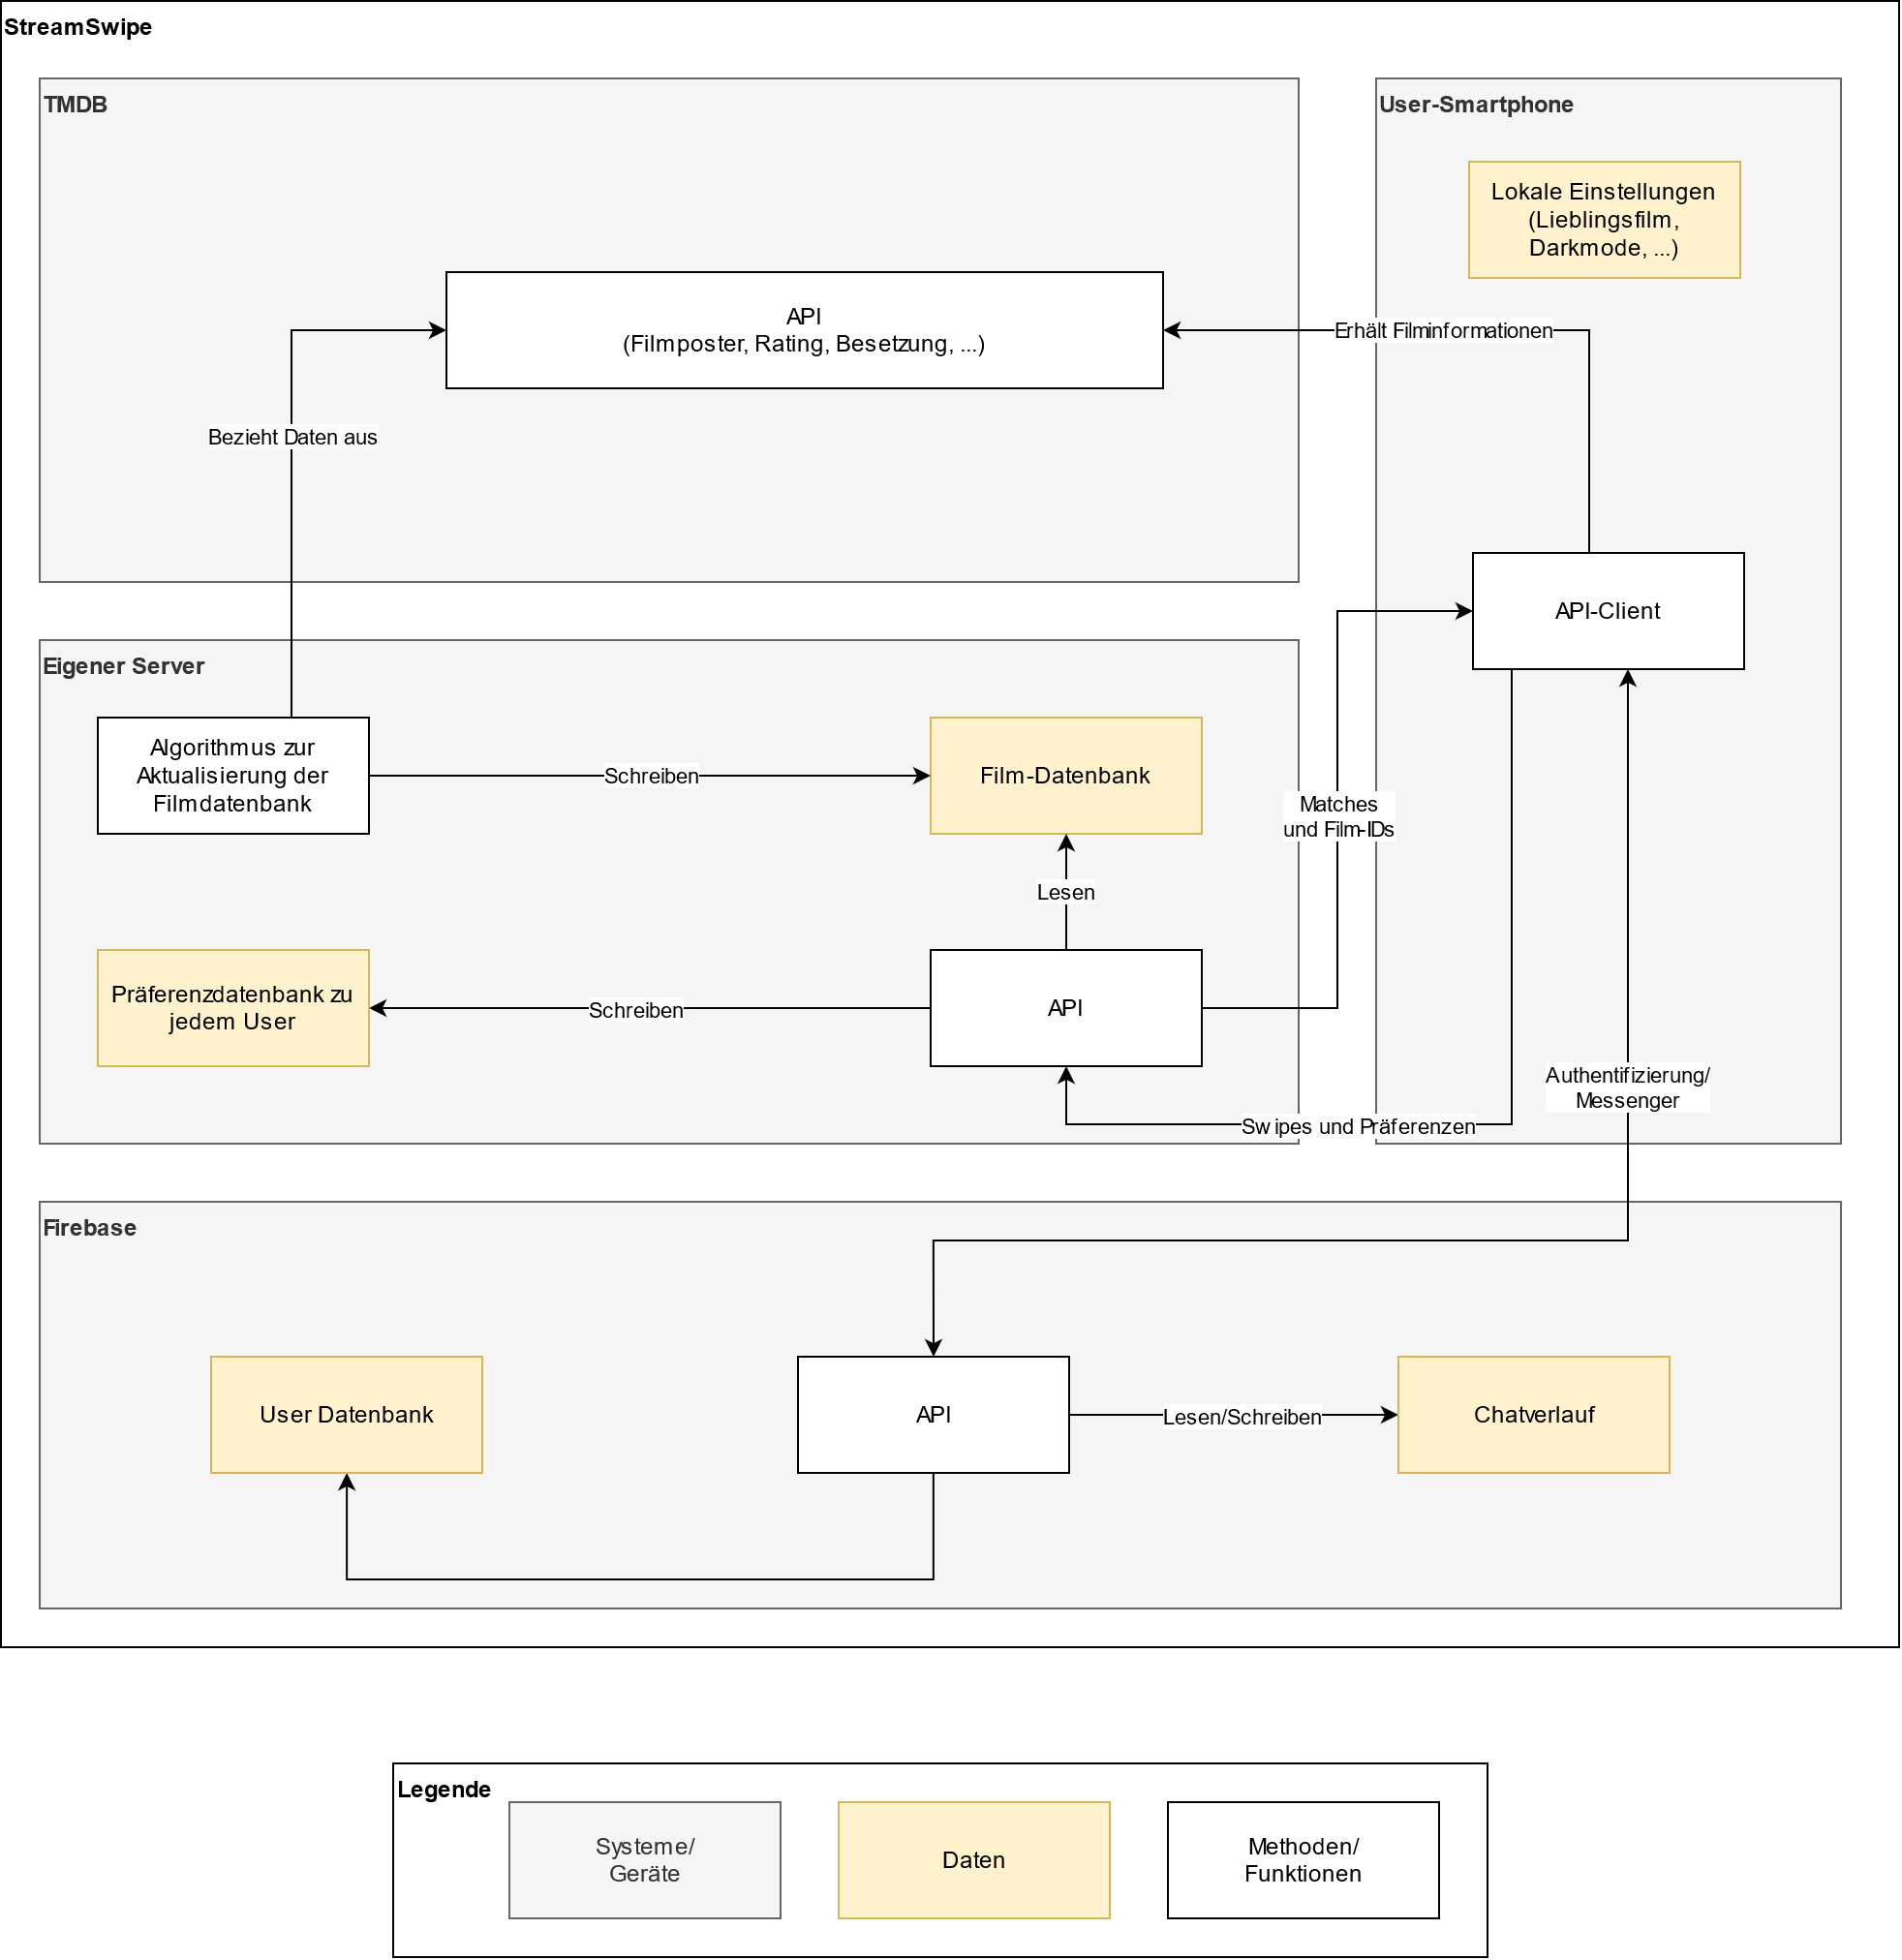
\includegraphics[width=16cm]{images/Konzeptdiagramm.png}
\caption{Komponentendiagramm}
\label{fig:komponentendiagramm}
\end{figure}









